\documentclass[12pt]{article}
\usepackage[a4paper, total={6in, 9in}]{geometry}
\usepackage{graphicx}
\graphicspath{ {./images/output/} }
\usepackage{caption}
\usepackage[english]{babel}
\usepackage{titling}
\usepackage{float}
% \usepackage{amsmath}
% \usepackage{minted}
% \usepackage{multicol}
% \usepackage{array}
% \usepackage{setspace}
% \usepackage{placeins}
% \usepackage{hyperref}
\setlength{\parindent}{0pt}

% \usepackage{lipsum}

\title{Drawing Line Diagrams in AutoCAD Electrical.}
\author{}
\date{}

\pagenumbering{gobble}
\begin{document}
\vspace*{\fill}
\begin{center}

    \emph{Heaven's Light is Our Guide} \\
    \textbf{Rajshahi University of Engineering and Technology} \\

    \begin{figure}[H]
        \centering
        
\includegraphics[scale=.34]{images/RUET_logo.png}
        \label{fig:ruet_logo}
    \end{figure}
    \vspace{5mm}

    \textbf{Course Code}\\
    ECE 3200\\
    \vspace{3mm}
    \textbf{Course Title}\\
    Electrical Services Design

    \vspace{5mm}
    \textbf{Experiment Date:} {February 4, 2025}\\
    \textbf{Submission Date:} {February 18, 2025}\\

    \vspace{5mm}
    \textbf{Lab Report 5: \\ Implementation of Parametric \& Full Units PLC: Insertion, Editing, \& Modification.}

    \vspace{15mm}

    \begin{tabular}{c|c}
        \textbf{Submitted to} & \textbf{Submitted by} \\
        Md. Faysal Ahamed     &                       \\
        Lecturer              &                       \\
        Dept of ECE, RUET     & Md. Tajim An Noor     \\
        -                     & Roll: 2010025         \\
        Moloy Kumar Ghosh     &                       \\
        Lecturer              &                       \\
        Dept of ECE, RUET     &                       \\
    \end{tabular}

\end{center}
\vspace*{\fill}


\pagebreak

\tableofcontents

\pagebreak
\pagenumbering{arabic}
\maketitle

\section*{Introduction}
\addcontentsline{toc}{section}{Introduction}
Line diagrams, or schematic diagrams, are crucial for clearly \& systematically representing electrical circuits. These diagrams use st\&ardized symbols to show the connections between various electrical components, such as switches, relays, motors, \& power sources.
\\\\
AutoCAD Electrical is a specialized tool designed to create \& manage electrical schematics with high precision \& efficiency. It offers a vast library of symbols, automated wire numbering, \& real-time error checking to simplify the design process.
\\\\
This experiment delves into the basic steps of drawing a line diagram using AutoCAD Electrical. It includes selecting appropriate symbols, arranging components correctly, wiring techniques, \& best practices for creating professional-quality schematics.
\\\\
The aim of this report is to deepen the underst\&ing of electrical design principles while building proficiency in using AutoCAD Electrical for practical electrical engineering applications.

\section*{Required Equipment/Software}
\addcontentsline{toc}{section}{Required Equipment/Software}
\begin{itemize}
    \item AutoCAD Electrical
    \item \LaTeX{} for report writing
\end{itemize}

\section*{Transmission \& Distribution Diagram}
\addcontentsline{toc}{section}{Transmission \& Distribution Diagram}
The transmission \& distribution of electrical power are essential processes for delivering electricity from power plants to consumers. Transmission involves the high-voltage transfer of electricity from generation stations to substations using transmission lines that typically operate between 69 kV \& 765 kV to reduce energy losses over long distances. Step-up transformers increase voltage for efficient long-distance travel, while step-down transformers at substations reduce voltage for distribution. Distribution delivers electricity from substations to residential, commercial, \& industrial users at lower voltages, typically between 230V \& 33kV. The distribution network includes feeders, distribution transformers, \& service lines, \& is divided into primary (medium voltage) \& secondary (low voltage) distribution to ensure safe \& reliable power delivery. In this lab, a line diagram will be created to illustrate the flow of electrical power from generation to consumers, highlighting key components such as transformers, transmission lines, substations, \& distribution feeders using AutoCAD Electrical.

\begin{figure}[H]
    \centering
    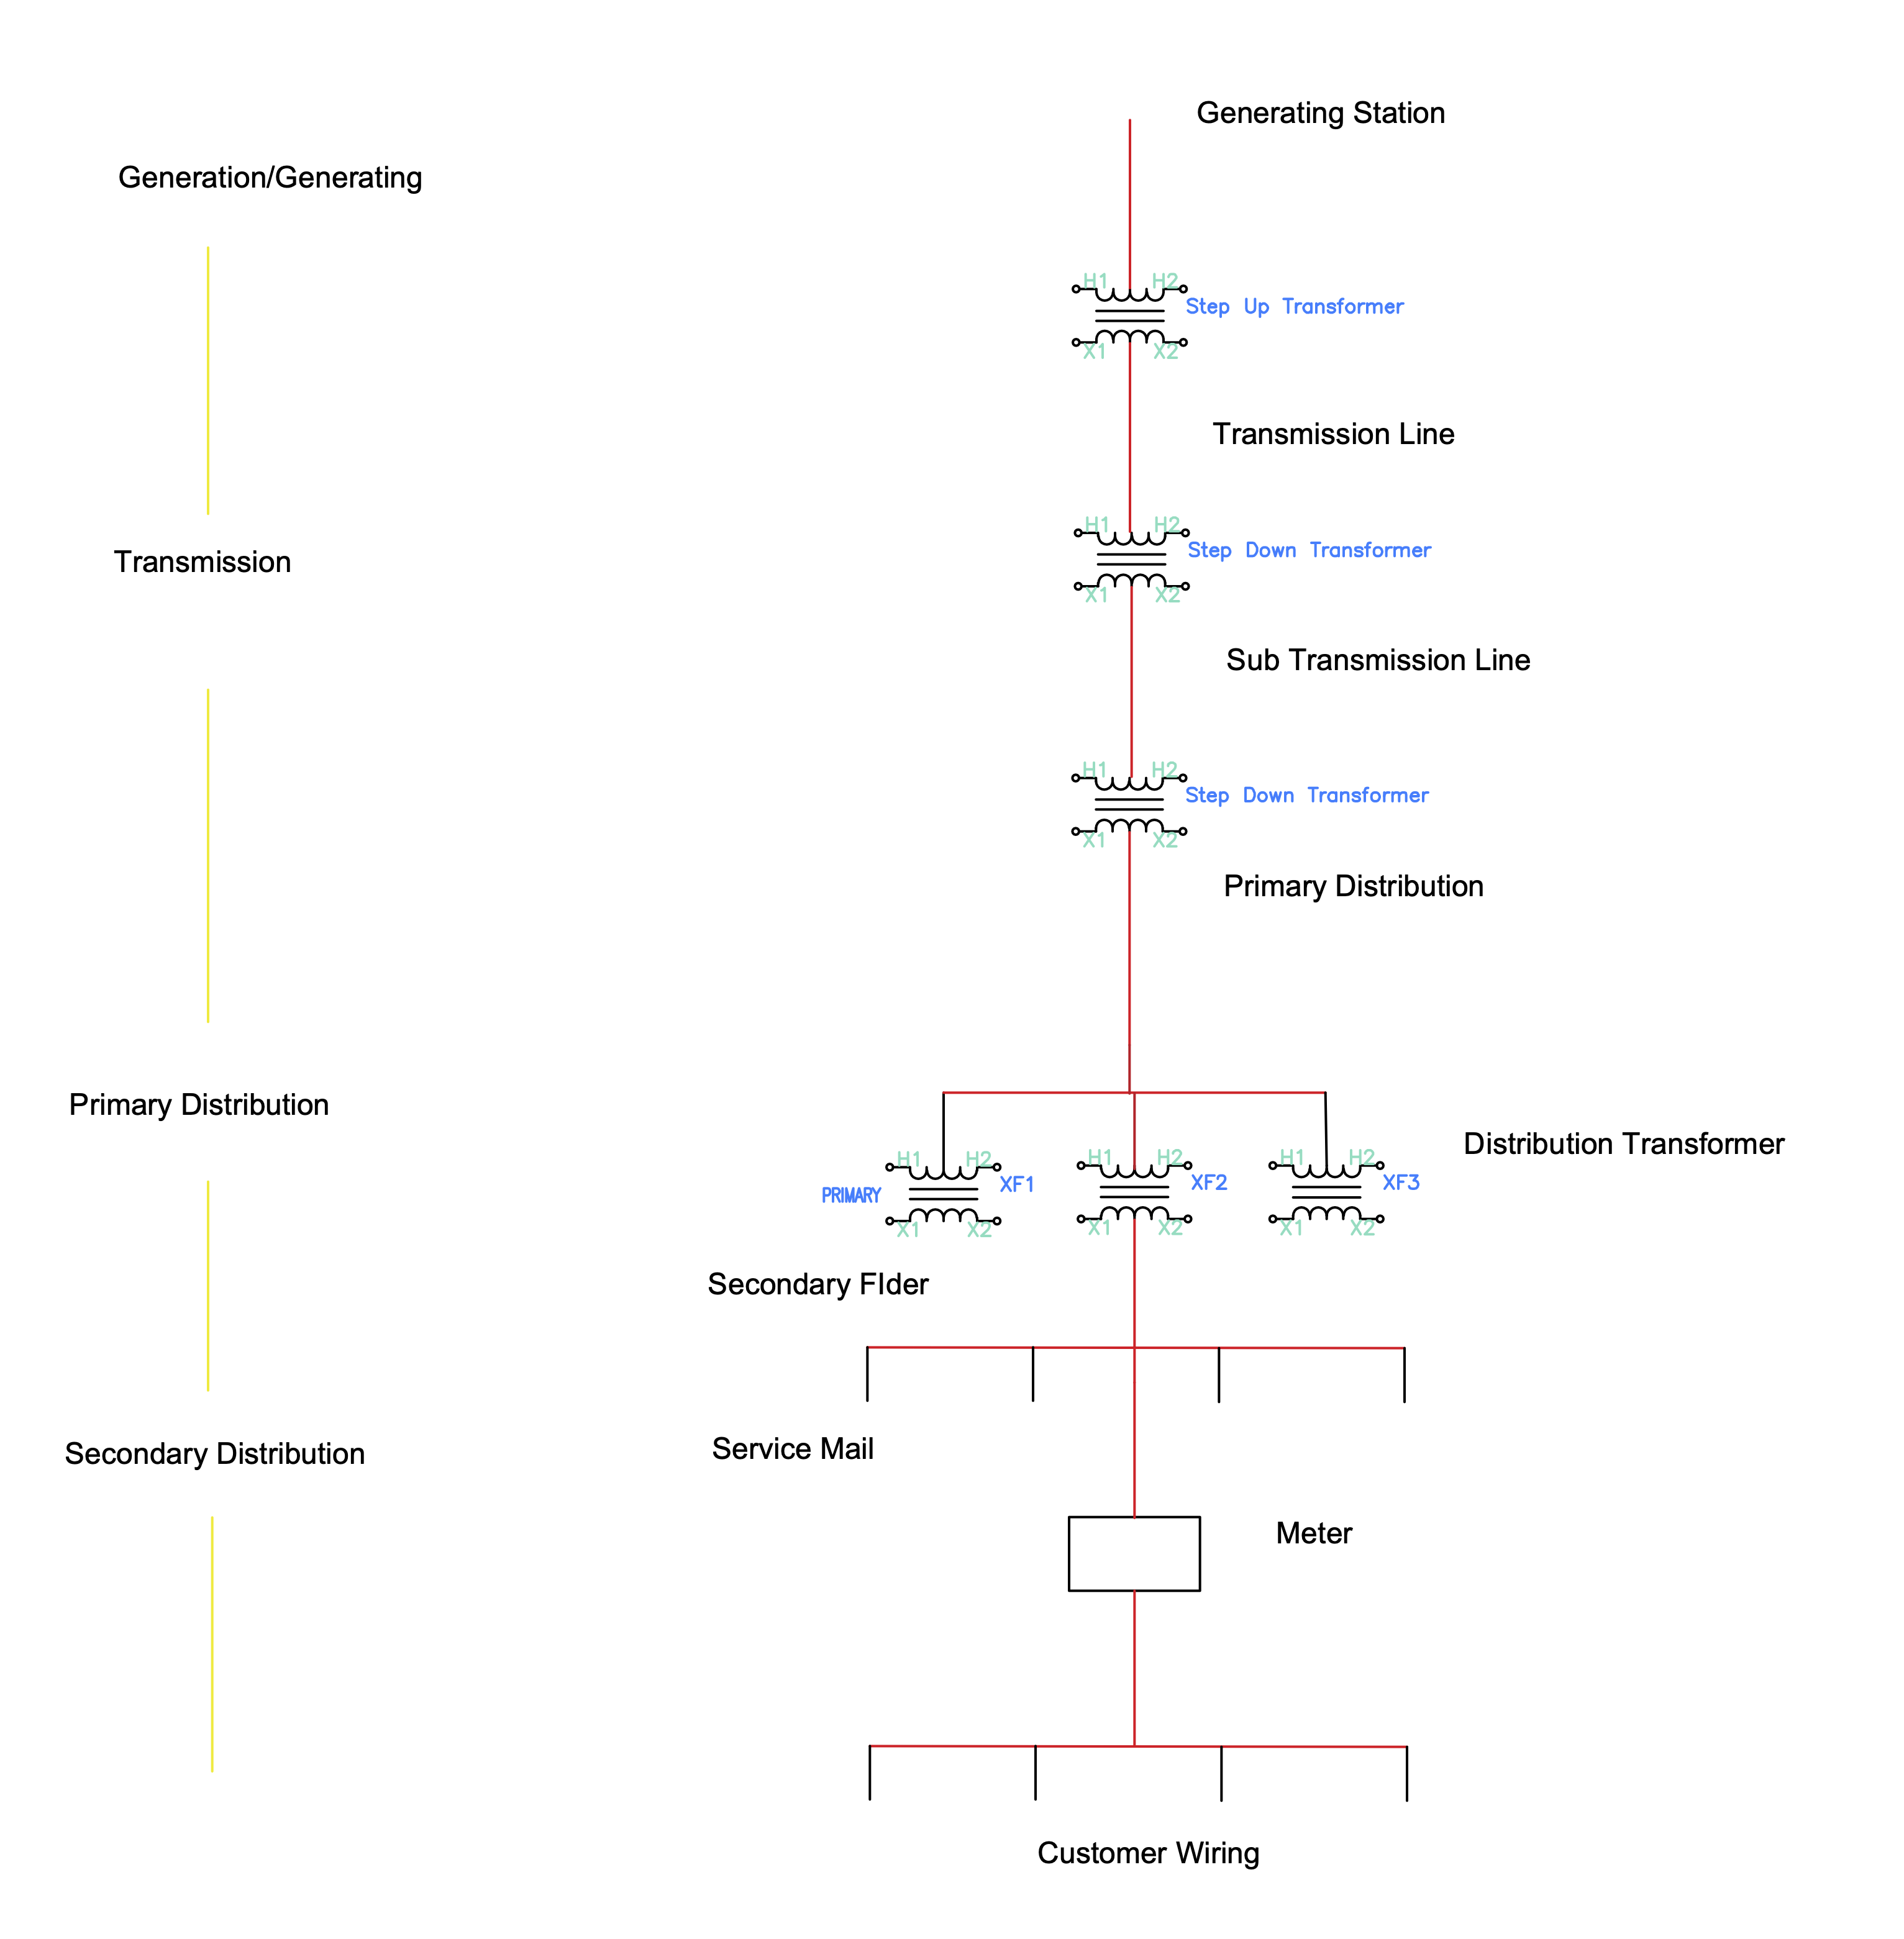
\includegraphics[width=\textwidth]{1.png}
    \caption{Transmission \& Distribution Diagram}
    \label{fig:transmission_distribution}
\end{figure}

\section*{11KV/230V Power Line Diagram}
\addcontentsline{toc}{section}{11KV/230V Power Line Diagram}
An 11kV/230V power line is a common step-down distribution system designed to deliver electricity to residential \& commercial areas. This system reduces the voltage from 11kV (medium voltage) to 230V (low voltage), ensuring it is safe for consumer use. Initially, power is transmitted at 11kV from the substation through distribution feeders. A step-down transformer (11kV/230V) then converts this voltage to 230V, which is subsequently distributed to homes, offices, \& small industries via service lines.

\begin{figure}[H]
    \centering
    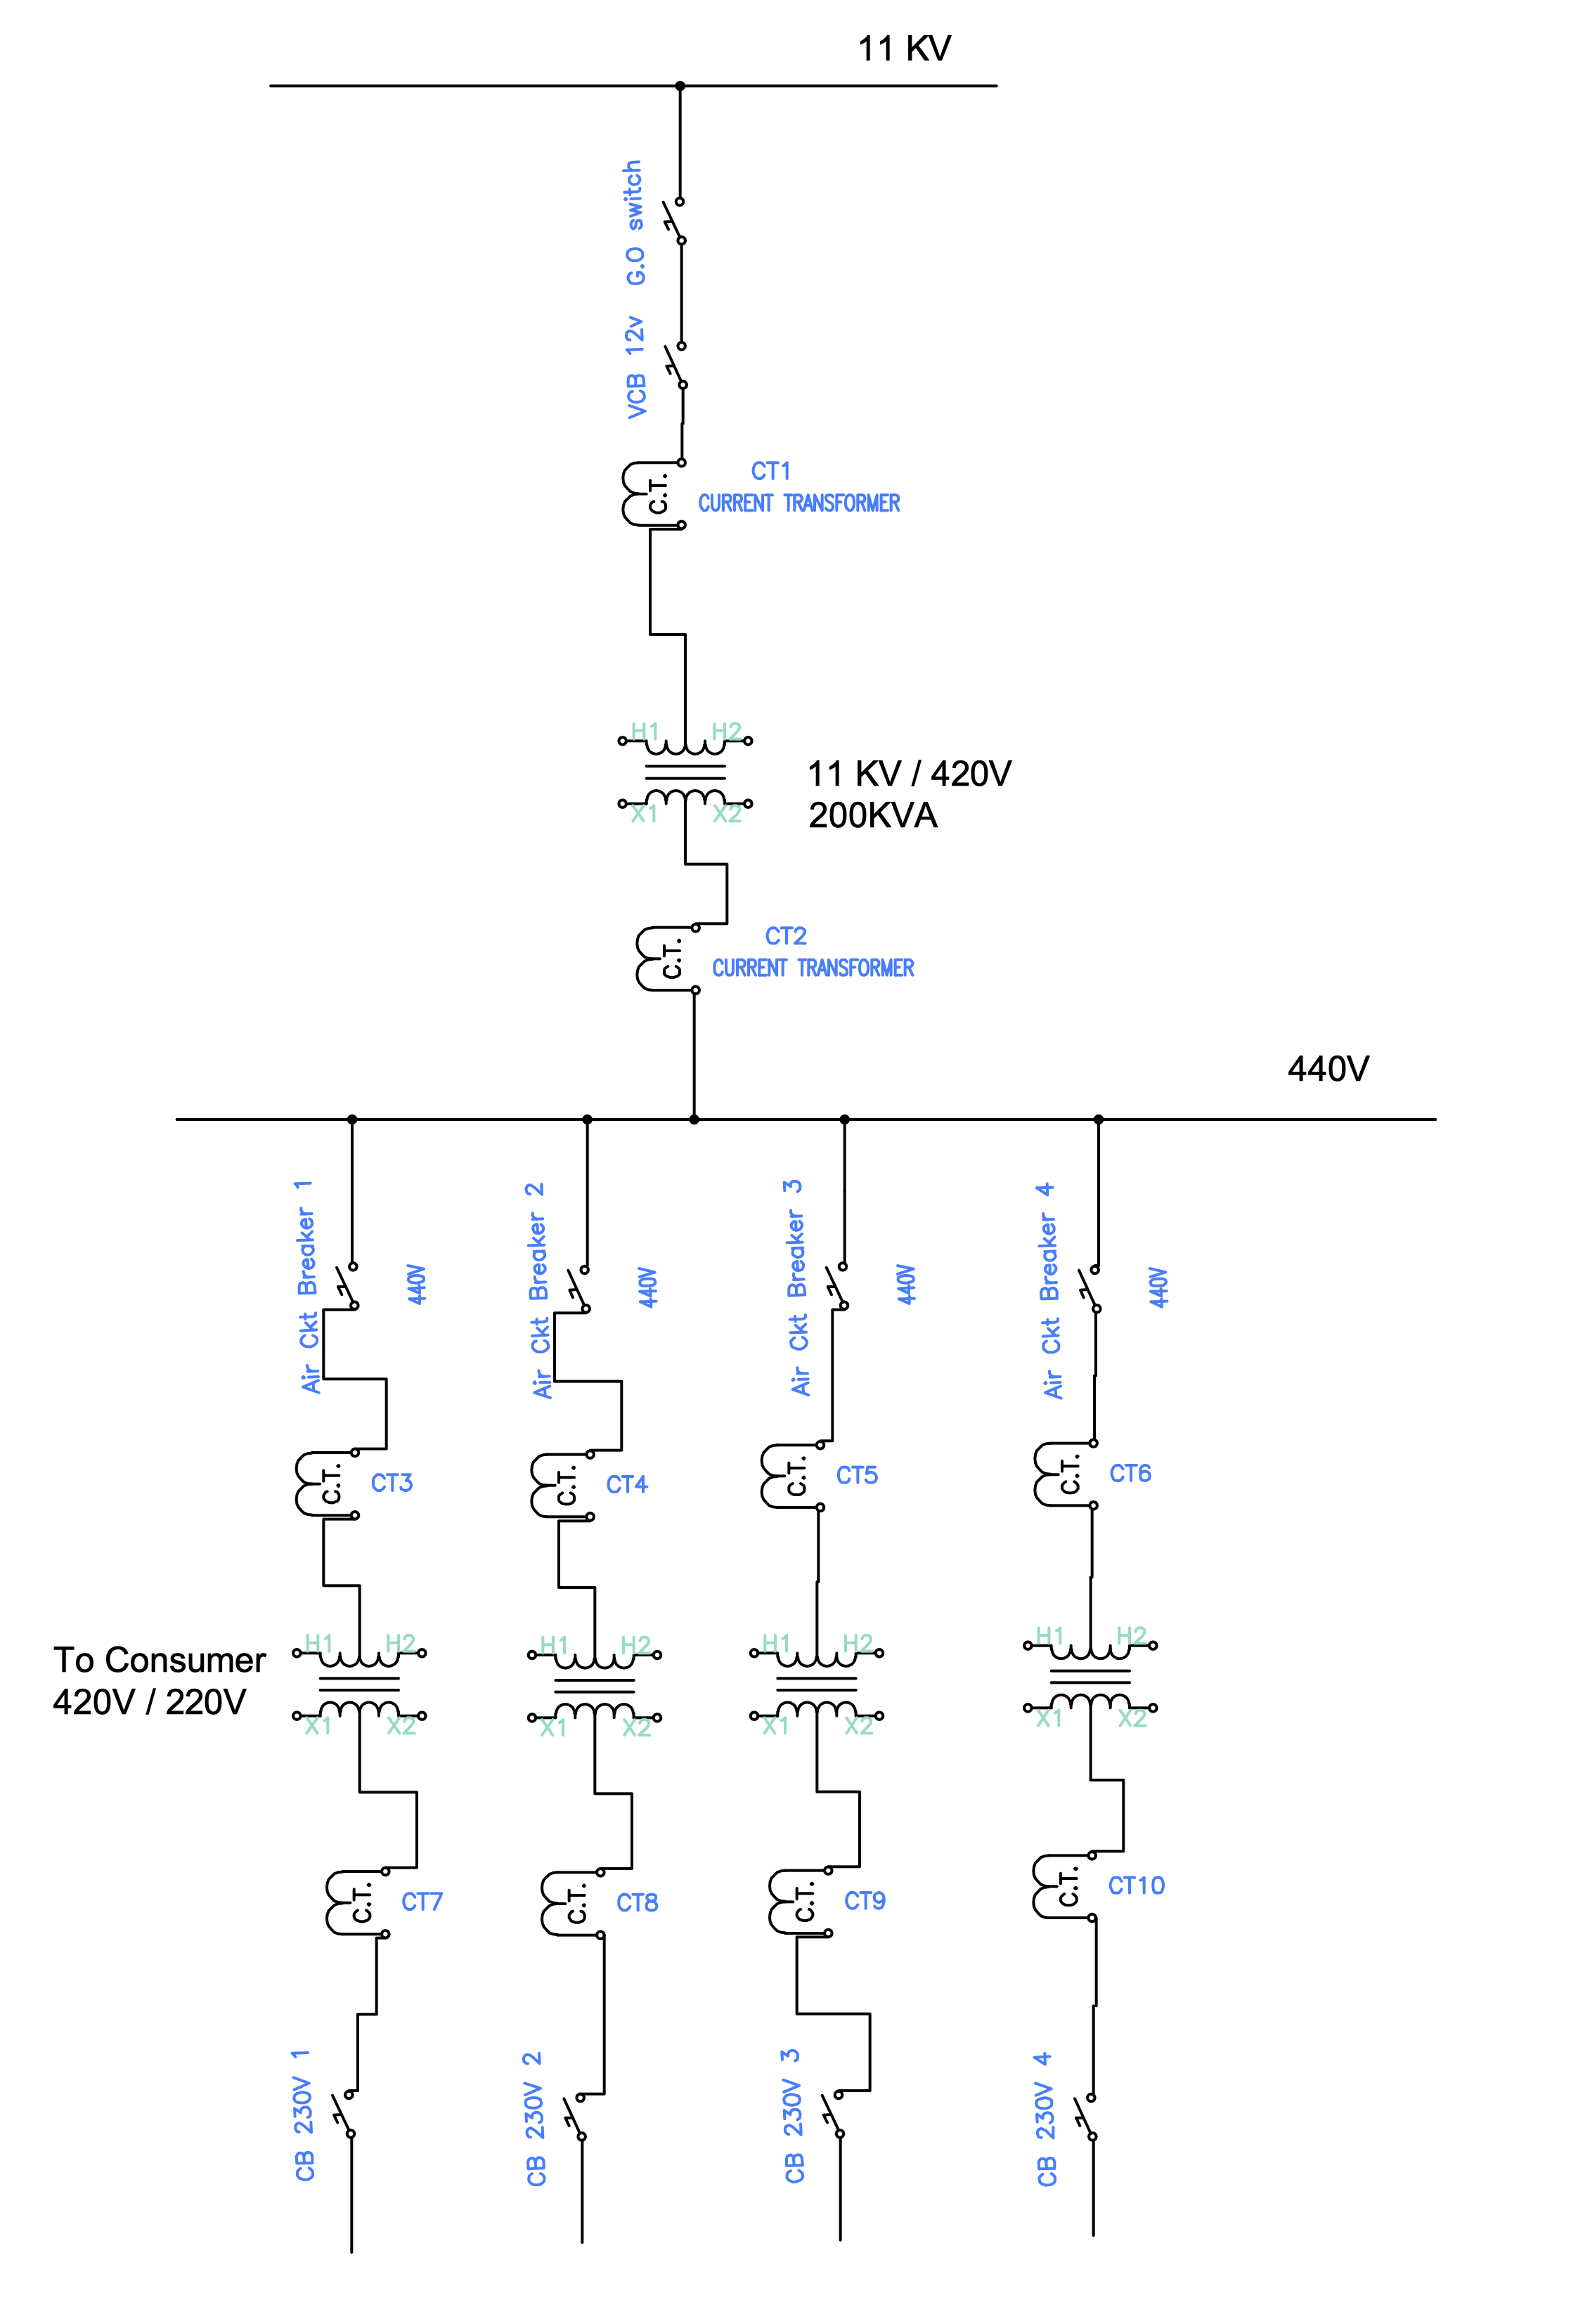
\includegraphics[width=.76\textwidth]{2.png}
    \caption{11KV/230V Power Line Diagram}
    \label{fig:power_line}
\end{figure}

\section*{Discussion \& Conclusion}
\addcontentsline{toc}{section}{Discussion \& Conclusion}
AutoCAD Electrical offers comprehensive tools for electrical design. Snap options ensure precise alignment, while ladder diagram settings aid systematic representation. The X-Y grid and X-Zones setup help organize the workspace. In this lab, we created line diagrams for transmission, distribution systems, and an 11kV/230V power line using AutoCAD Electrical. We selected symbols, arranged components, and ensured proper wiring techniques. Automated features like wire numbering and real-time error checking streamlined the process and minimized errors.
\\\\
The transmission and distribution diagram illustrated how electrical power is transferred from generation to consumers, emphasizing the role of transformers in managing voltage levels. The 11kV/230V power line diagram showed the practical application of these principles in residential and commercial systems. This lab reinforced electrical service design concepts and demonstrated AutoCAD Electrical's capabilities. Mastering this tool is crucial for accurate and efficient electrical designs, enhancing design quality and system reliability.

% \bibliographystyle{IEEEtran}
% \renewcomm\&{\bibname}{References}
% \addcontentsline{toc}{section}{References}
% \bibliography{ref}

\end{document}
